% !Rnw weave = knitr
% !TeX program = pdfLaTeX
\documentclass[a4paper,10pt]{article}\usepackage[]{graphicx}\usepackage[]{xcolor}
% maxwidth is the original width if it is less than linewidth
% otherwise use linewidth (to make sure the graphics do not exceed the margin)
\makeatletter
\def\maxwidth{ %
  \ifdim\Gin@nat@width>\linewidth
    \linewidth
  \else
    \Gin@nat@width
  \fi
}
\makeatother

\definecolor{fgcolor}{rgb}{0.345, 0.345, 0.345}
\newcommand{\hlnum}[1]{\textcolor[rgb]{0.686,0.059,0.569}{#1}}%
\newcommand{\hlstr}[1]{\textcolor[rgb]{0.192,0.494,0.8}{#1}}%
\newcommand{\hlcom}[1]{\textcolor[rgb]{0.678,0.584,0.686}{\textit{#1}}}%
\newcommand{\hlopt}[1]{\textcolor[rgb]{0,0,0}{#1}}%
\newcommand{\hlstd}[1]{\textcolor[rgb]{0.345,0.345,0.345}{#1}}%
\newcommand{\hlkwa}[1]{\textcolor[rgb]{0.161,0.373,0.58}{\textbf{#1}}}%
\newcommand{\hlkwb}[1]{\textcolor[rgb]{0.69,0.353,0.396}{#1}}%
\newcommand{\hlkwc}[1]{\textcolor[rgb]{0.333,0.667,0.333}{#1}}%
\newcommand{\hlkwd}[1]{\textcolor[rgb]{0.737,0.353,0.396}{\textbf{#1}}}%
\let\hlipl\hlkwb

\usepackage{framed}
\makeatletter
\newenvironment{kframe}{%
 \def\at@end@of@kframe{}%
 \ifinner\ifhmode%
  \def\at@end@of@kframe{\end{minipage}}%
  \begin{minipage}{\columnwidth}%
 \fi\fi%
 \def\FrameCommand##1{\hskip\@totalleftmargin \hskip-\fboxsep
 \colorbox{shadecolor}{##1}\hskip-\fboxsep
     % There is no \\@totalrightmargin, so:
     \hskip-\linewidth \hskip-\@totalleftmargin \hskip\columnwidth}%
 \MakeFramed {\advance\hsize-\width
   \@totalleftmargin\z@ \linewidth\hsize
   \@setminipage}}%
 {\par\unskip\endMakeFramed%
 \at@end@of@kframe}
\makeatother

\definecolor{shadecolor}{rgb}{.97, .97, .97}
\definecolor{messagecolor}{rgb}{0, 0, 0}
\definecolor{warningcolor}{rgb}{1, 0, 1}
\definecolor{errorcolor}{rgb}{1, 0, 0}
\newenvironment{knitrout}{}{} % an empty environment to be redefined in TeX

\usepackage{alltt}
\usepackage[utf8]{inputenc}
\usepackage[T1]{fontenc}
\usepackage[french]{babel}
\usepackage{csquotes}
\usepackage{hyperref}
\usepackage{xcolor}

% Booktabs
\usepackage{booktabs}

% Géométrie
\usepackage{geometry}
\geometry{
a4paper, 
total={170mm,257mm},
left=20mm,
top=15mm}

% Maths
\usepackage{amsmath}
\DeclareMathOperator*{\argmax}{argmax}
\DeclareMathOperator*{\argmin}{argmin}
\usepackage{amsfonts}
\usepackage{dsfont}
\usepackage{bm}

% Images 
\usepackage{wrapfig}
\usepackage{graphicx}
\graphicspath{ {./images/} }

% Citations et biblio
\usepackage[backend=biber, style=apa]{biblatex}
%== use and define color ==%
%\usepackage[style=numeric,backend=biber,doi=false,isbn=false,max
\AtEveryCite{\color{blue}}
\addbibresource{references.bib}


% Commande pour les nombres réels
\newcommand{\R}{\mathbb{R}}
\newcommand{\segspace}{\mathcal{T}_K}

% Commande pour les entiers naturels
\newcommand{\N}{\mathbb{N}}

% Commande pour les entiers relatifs
\newcommand{\Z}{\mathbb{Z}}

% Commande pour les nombres complexes
\newcommand{\C}{\mathbb{C}}

% Commande pour la probabilité
\newcommand{\Prob}{\mathbb{P}}

% Commande pour l'espérance
\newcommand{\E}{\mathbb{E}}

% Commande pour la variance
\newcommand{\Var}{\text{Var}}

% Commande pour la covariance
\newcommand{\Cov}{\text{Cov}}

% Commande pour la convergence en probabilité
\newcommand{\convprob}{\xrightarrow{P}}

% Commande pour la convergence en loi
\newcommand{\convloi}{\xrightarrow{d}}

% Commande pour la convergence en moyenne quadratique
\newcommand{\convmq}{\xrightarrow{L^2}}

% Poisson
\newcommand{\Poisson}[1]{\mathcal{P} ({#1})}

% Pagination
\usepackage{fancyhdr}
\pagestyle{fancy}
% Place Page X of Y on the right-hand
% side of the footer
\fancyhf{}
\rfoot{\thepage}

\title{\vspace{-1.5cm}\large Détection de ruptures dans des processus de Poisson - Stéphane Robin\\
\small Compte-rendu du séminaire\vspace{-0.5cm}}
\date{\small 30 Jan. 2024}
\author{\small Louis Lacoste}



\IfFileExists{upquote.sty}{\usepackage{upquote}}{}
\begin{document}
\maketitle

\section{Introduction}

\begin{wrapfigure}[14]{L}{0.27\textwidth}
    \centering
    \vspace{-5pt}
    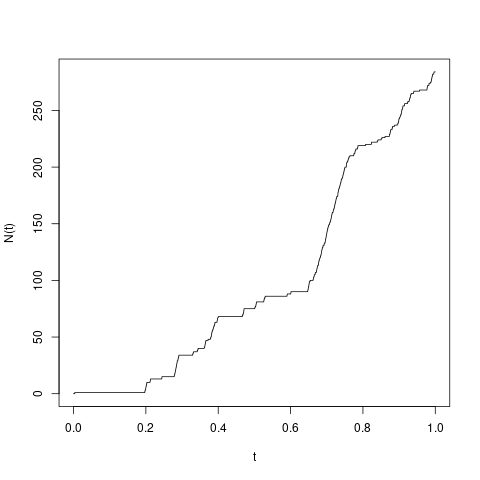
\includegraphics[width=0.27\textwidth]{graph-cris-chauve-souris}
    \vspace{-20pt}
    \caption{\small Comptage de cris de chauve-souris (nuit du 17 juillet 2019)}
    \label{fig:graph-cris-chauve-souris}
\end{wrapfigure}

Stéphane Robin nous présente une méthode qu'ils ont développé avec Emilie Lebarbier
et Charlotte Dion-Blanc. Cette méthode est présentée dans l'article 
\cite{dion-blancDetectionRupturesMultiples2023} sur HAL.

\begin{wrapfigure}[14]{R}{0.27\textwidth}
    \centering
    \vspace{-20pt}
    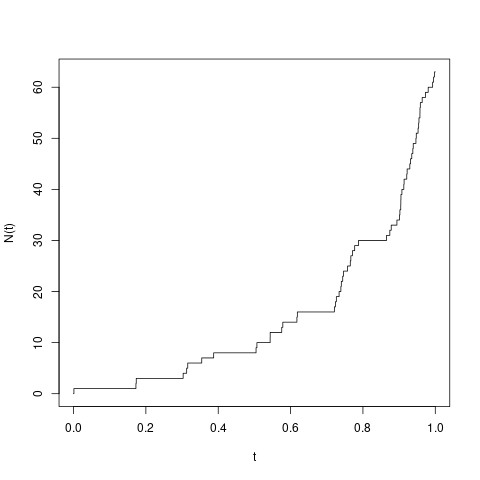
\includegraphics[width=0.27\textwidth]{graph-eruption-kilauea}
    \vspace{-20pt}
    \caption{Données d'éruption du Kilauea, 1750 - 1984}
    \label{fig:graph-eruption-kilauea}
\end{wrapfigure}

La méthode considère des données de comptages au cours du temps. Un exemple de 
telles données est celui du nombre de cris de chauve-souris au cours de la nuit.
Ces données sont présentées dans sur la figure~\ref{fig:graph-cris-chauve-souris}.
Ou encore les données d'éruption du volcan Kilauea présentée sur la figure~\ref{fig:graph-eruption-kilauea}.

L'intervalle de temps est normalisé, $t\in[0,1]$ et les instants d'évènements 
sont les $0<T_1<\dots T_i<\dots T_n < 1$.
Étant donné qu'il s'agit d'un comptage aléatoire, le processus \emph{naturel}
est le processus de comptage, $N(t) = \sum_{i=1}^n \mathds{1}_{T_i \leq t}$ et 
parmi les processus de comptage, le processus de Poisson défini par sa fonction 
d'intensité $\lambda(t)$.\\

\section{Méthode}

La méthode fait l'hypothèse que la fonction d'intensité est constante par 
morceaux et qu'il existe des \emph{points de ruptures} les $(\tau_k)_{0\leq k \leq K}$.
Et alors pour $t \in I_k = ] \tau_{k-1}; \tau_{k} ], \lambda(t) = \lambda_k$.
Ainsi l'objectif de la méthode est d'estimer les paramètres 
$\theta =((\tau_k)_{0\leq k \leq K}, (\lambda_k)_{0\leq k \leq K} )$ et de 
réaliser une \emph{sélection de modèle} pour obtenir le nombre de segments $K$.

\subsection{Segmentation}

Un rappel sur la segmentation en temps discret, nous montre que la programmation
dynamique permet ainsi de résoudre le problème d'estimation des paramètres dans 
ce cas qui semblait apparemment computationnellement complexe.

Dans le cas de la méthode, le problème d'optimisation est 
$$(\widehat{\bm{\tau}}, \widehat{\bm{\lambda}}) = 
\argmin_{\bm{\tau}\in\segspace, \bm{\lambda} \in (\R^+)^K} \gamma (\bm{\tau}, \bm{\lambda})$$

L'additivité du contraste: $\gamma(\bm\tau, \bm\lambda) = 
\sum_{k=1}^K C(\Delta N_k, \Delta\tau_k, \lambda_k)$ en tant que somme sur les 
segments aide à la résolution du problème d'optimisation.
En effet le $\bm \lambda = (\lambda_1, \dots, \lambda_K)$ optimal peut être obtenu grâce à la propriété d'additivité
en résolvant $\widehat \lambda_k = \lambda_k (\tau) = \argmin_{\lambda_k \in \R^+} 
C(\Delta N_k, \Delta\tau_k)$.
Et si la fonction de contraste est la log-vraisemblance négative, on a : 
$\widehat \lambda_k = \Delta N_k / \Delta \tau_k$.

Mais le problème difficile est celui de trouver le $\bm\tau = (\tau_0, \dots, 
\tau_K)$ optimal, car le problème 
d'optimisation est alors $\widehat \tau = 
\argmin_{\tau\in\segspace} \widehat \gamma(\tau), 
\widehat \gamma(\tau) = \gamma (\tau, \widehat \lambda (\tau))$ où $\segspace$ 
est l'espace de segmentation \textbf{continu}, $$\segspace = 
\bigl\{ \tau \in [0,1]^{K+1} : 0 = \tau_0 < \tau_1 \dots < \tau_{K-1} < 
\tau_K = 1 \bigr\}$$

Car le contraste n'est ni convexe ni continu par rapport à $\tau$.

La figure~\ref{fig:contrast-function} présente les valeurs de la fonction de 
contraste pour les paramètres donnés. Sur la figure, chaque "bloc" correspond à
une partition des nombre d'évènements ($\Delta N = (\Delta N_1, \Delta N_2, 
\Delta N_3)$.

L'idée est alors de partitionner le nombre d'évènements  $\mathcal{N} = 
\bigl\{ \nu \in \N^K : \sum_{k=1}^K \nu_k = n \bigr\}$ où $\nu_k$ est le nombre
d'évènements dans le segment k. Puis à partir de cette partition, on peut 
partitionner l'espace de segmentation $\mathcal{T}(\nu) = 
\bigl\{ \bm \tau \in \segspace : \Delta N = \nu \bigr\}$ qui satisfait la 
partition $\nu$. Ce qui permet de réécrire le problème de minimisation :
$$\min_{\bm{\tau}\in\segspace} \widehat \gamma (\bm{\tau}) = \min_{\nu \in 
\mathcal{N}^K} \min_{\bm{\tau}\in\mathcal{T}(\nu)} \widehat \gamma (\bm{\tau})$$

\newpage

\begin{wrapfigure}[21]{L}{0.25\textwidth}
    \centering
    \caption{Fonction de contraste et partitionnement de l'espace pour $n=10$, $K=3$ et $\tau = (\tau_1,\tau_2)$}
    \label{fig:contrast-function}
    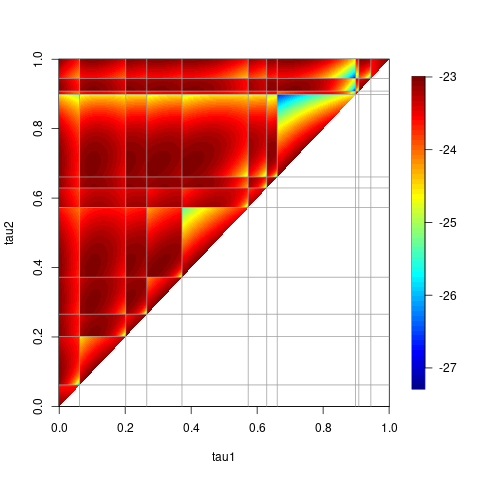
\includegraphics[width=0.25\textwidth]{contrast-function}
    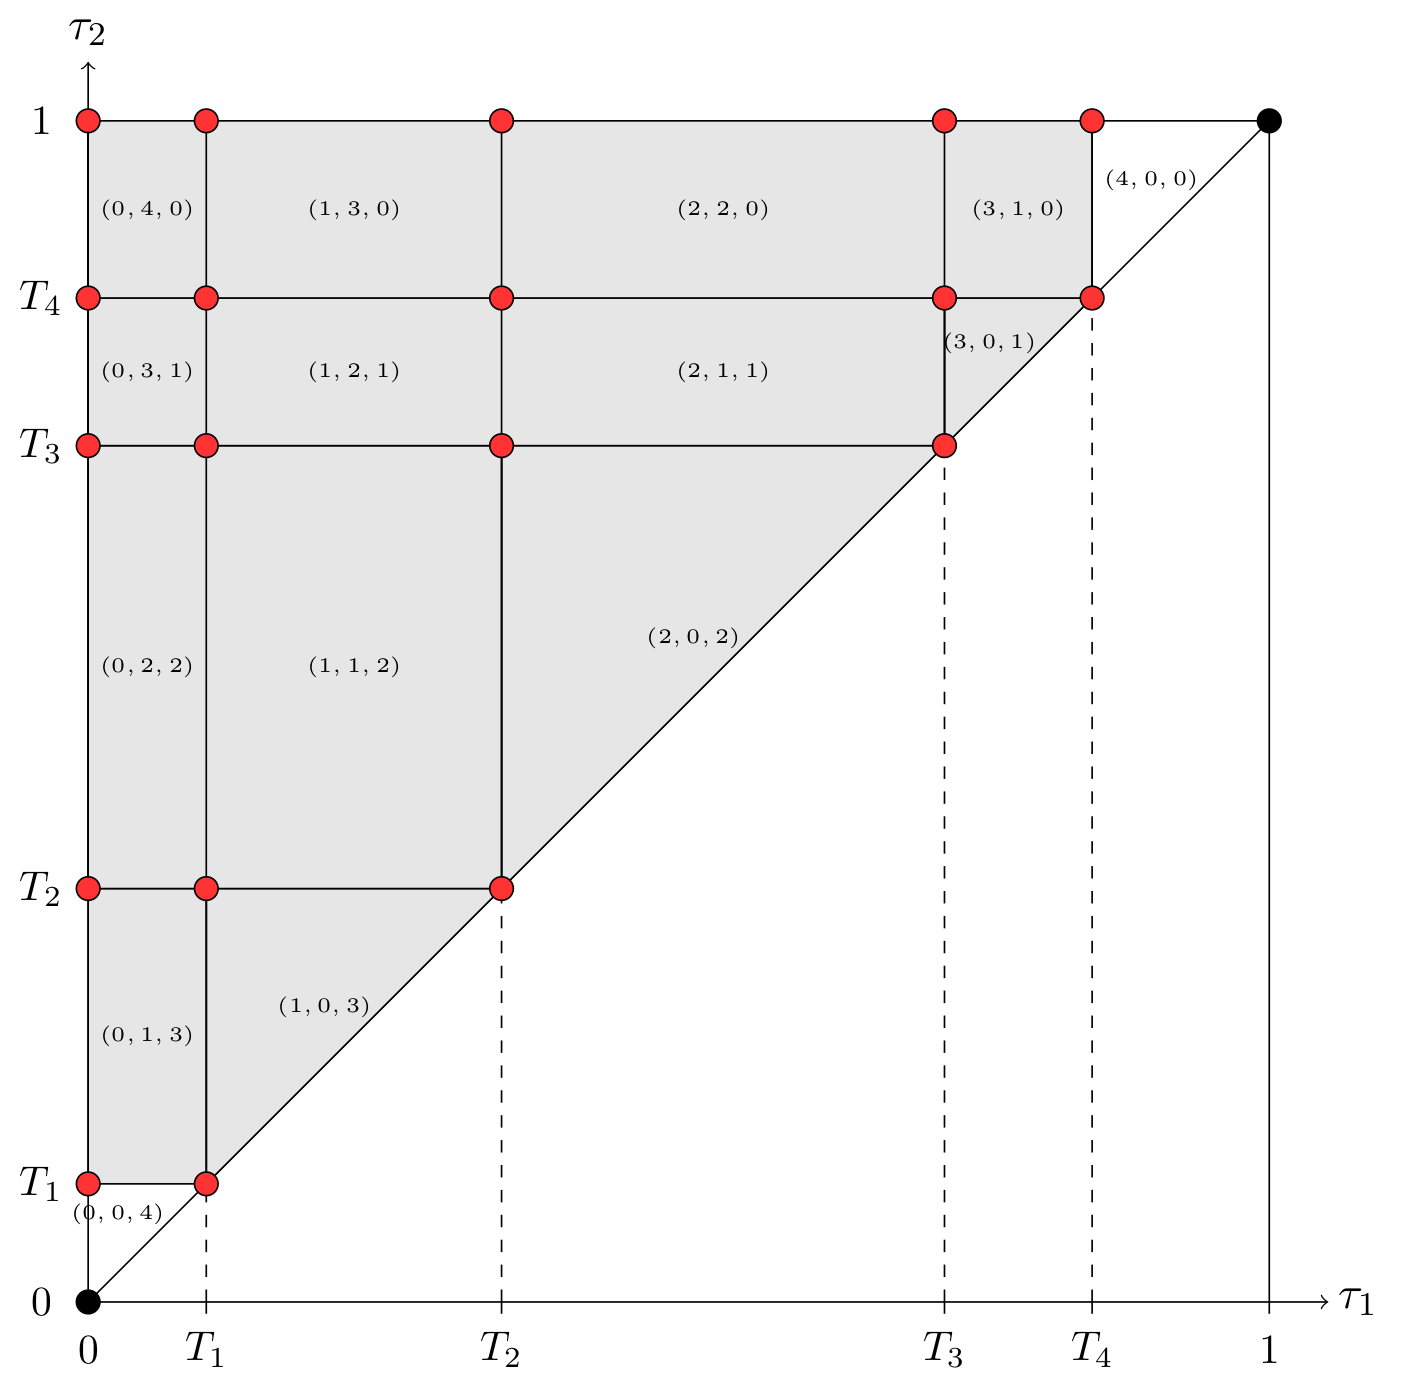
\includegraphics[width=0.25\textwidth]{space-partitioning}
\end{wrapfigure}

Et alors grâce aux propriétés de stricte concavité des fonctions de coût $C$ par
rapport aux $\Delta \tau_k$ les auteurs montrent que $\hat{\tau} = 
\argmin_{\tau\in\segspace} \hat{\gamma}(\bm{\tau}) \subset \bigl\{ T^-_1, T_1, 
\dots, T^-_n, T_n \bigr\}$\footnote{$T_i^-$ représente l'instant juste avant le saut
au temps $T_i$.}. Et ainsi, la programmation dynamique permet de trouver
les points de ruptures avec une complexité $\mathcal{O}(n^2)$.

Un contraste concave par rapport à $\Delta\tau$ est dit admissible (par exemple
les contrastes de Poisson et Poisson-Gamma). Et un contraste est dit désirable
n'autorise pas les segments de longueur nulle (et c'est le cas du 
Poisson-Gamma).

\subsection{Sélection de modèle}

Pour la sélection de modèle la propriété de \emph{thinning} du processus de 
Poisson permet d'obtenir deux processus de Poisson indépendants et donc 
de pouvoir faire de la \emph{cross-validation}

\subsection{Extension : Processus de Poisson marqué}

Le processus de Poisson marqué est une extension et la méthode de détection de
rupture peut gérer ces données supplémentaires.

Un processus de Poisson est dit marqué si à chaque temps de saut $T_i$ est 
associé une "marque". Pour l'exemple des volcans, il s'agit de la durée de l'
éruption et pour les cris de chauve-souris, il peut s'agir soit de l'espèce ou 
encore de la durée du cri.

Mathématiquement, cela peut se noter : 
$$(Y(t))_{0\leq t \leq 1} \sim MPP(\lambda(t), \mu(t)),$$ 
qui consiste en deux composantes :
$$(N(t))_{0\leq t \leq 1} \sim PP(\lambda(t)), X_i \sim \underbrace{\mathcal{F}}_{\text{loi de probabilité}}(\mu(T_i))$$

Et dans la présentation, on peut ainsi voir que sur un exemple d'éruption de 
l'Etna, la prise en compte des marques modifie l'estimation des paramètres. Ce 
qui dans le cas du volcan pourrait indiquer des modifications de son activité
sous-jacente.

\section{Apport personnel}



Nous allons tout d'abord simuler un processus de Poisson inhomogène\footnote{Le 
code pour ce rapport est disponible sur 
\url{https://github.com/Polarolouis/msv-seminaire-detction-rupture-processus-poisson}} selon les 
conditions du modèle et voir ce que donne l'estimation avec le package 
\texttt{CptPointProcess}.




La figure~\ref{fig:donnees-simu} présente les données simulées selon les 
paramètres suivants :
$$ \lambda = (1, 3, 10, 3), \text{ } \Delta N = (20, 20, 20, 20)
\text{ et } N(1) = 80 $$

\subsection*{Application de la méthode à données simulées}

\subsubsection*{En donnant le nombre de segments}

En fixant $K_{max} = 4$ et avec \texttt{selection = FALSE}. La méthode 
trouve donc les résultats suivant présentés dans la table~\ref{tab:resultat}.



\begin{table}[!h]
    \parbox{.45\linewidth}{
        \small
        \centering
\begin{knitrout}
\definecolor{shadecolor}{rgb}{0.969, 0.969, 0.969}\color{fgcolor}
\begin{tabular}{rrrrrl}
\toprule
begin & end & Dt & DN & lambda & code.end\\
\midrule
0.00 & 0.58 & 0.58 & 20 & 35.28 & -\\
0.58 & 0.74 & 0.15 & 19 & 120.64 & -\\
0.74 & 0.79 & 0.05 & 20 & 310.92 & .\\
0.79 & 1.00 & 0.21 & 20 & 94.55 & .\\
\bottomrule
\end{tabular}

\end{knitrout}
        \caption{Résultats de la méthode en donnant le nombre de segment}
        \label{tab:resultat}
    }
    \hfill
    \parbox{.45\linewidth}{
        \centering
        \small
\begin{knitrout}
\definecolor{shadecolor}{rgb}{0.969, 0.969, 0.969}\color{fgcolor}
\begin{tabular}{rrrrrl}
\toprule
begin & end & Dt & DN & lambda & code.end\\
\midrule
0.00 & 0.58 & 0.58 & 20 & 35.28 & -\\
0.58 & 0.66 & 0.07 & 16 & 194.93 & .\\
0.66 & 0.74 & 0.08 & 3 & 43.84 & -\\
0.74 & 0.79 & 0.05 & 20 & 310.92 & .\\
0.79 & 1.00 & 0.21 & 20 & 94.55 & .\\
\bottomrule
\end{tabular}

\end{knitrout}
        \caption{Résultats de la méthode en \emph{cross-validation}}
        \label{tab:resultat-cv}
    }
\end{table}

\begin{wrapfigure}{R}{0.27\textwidth}
    \centering
\begin{knitrout}
\definecolor{shadecolor}{rgb}{0.969, 0.969, 0.969}\color{fgcolor}
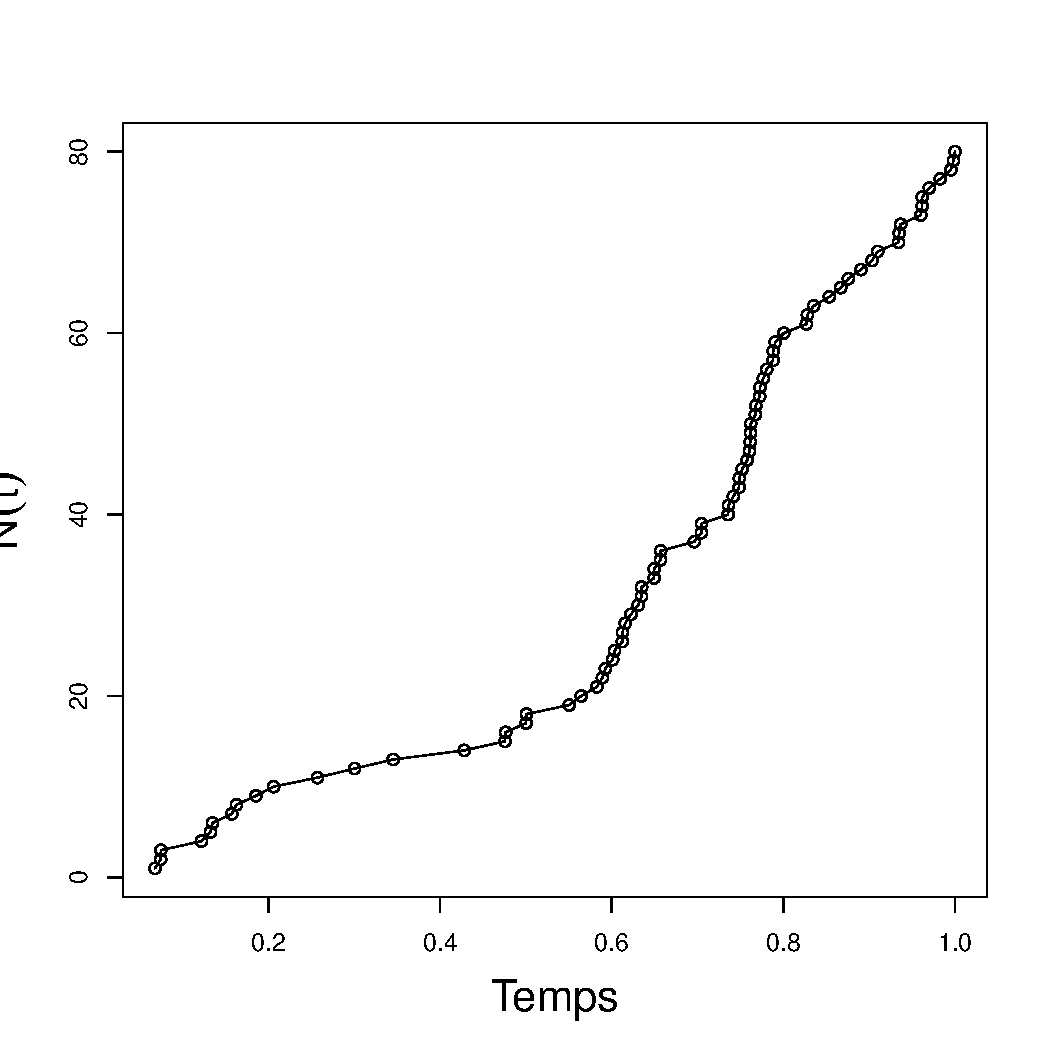
\includegraphics[width=0.27\textwidth,height=0.2\textheight]{figure/plot-1} 
\end{knitrout}
    \vspace{-10pt}
    \caption{Processus de Poisson inhomogène simulé}
    \label{fig:donnees-simu}
\end{wrapfigure}

Soit pour $\lambda = (0.96, 3.27, 8.43, 2.56)$
en \textbf{re-divisant par le temps maximal utilisé pour normaliser}.
Et on peut donc constater que la méthode parvient à retrouver les valeurs des 
différents paramètres. 

\subsubsection*{En sélectionnant $\hat{K}$ avec la \emph{cross-validation}}
En fixant seulement \texttt{selection = TRUE}. La méthode trouve donc les résultats suivant présentés dans la 
table~\ref{tab:resultat-cv}.

Soit pour $\lambda = (0.96, 5.29, 1.19, 8.43, 2.56)$.

\textbf{Remarque :} pour $K = 4$ et $N(1) = 
80$, l'estimation de $\hat{K}$ est un peu hors des clous,
mais nous avons testé en augmentant le nombre d'évènements. On peut imaginer que
le \emph{thinning} peut augmenter la variabilité, avec l'effet attendu en 
diminuant le nombre données.\\

On peut donc voir que si la méthode sélectionne correctement le nombre de 
segment l'estimation de paramètres obtenue est alors bonne, même pour un faible
nombre de données.

% \subsection*{Analyse de la sensibilité de la méthode à la quantité de 
% données par simulations}

\subsection*{Analyse de données de \cite{soubeyrandDonneesTheseExperience2024}}


\begin{wrapfigure}[12]{l}{0.27\textwidth}
    \centering
\begin{knitrout}
\definecolor{shadecolor}{rgb}{0.969, 0.969, 0.969}\color{fgcolor}
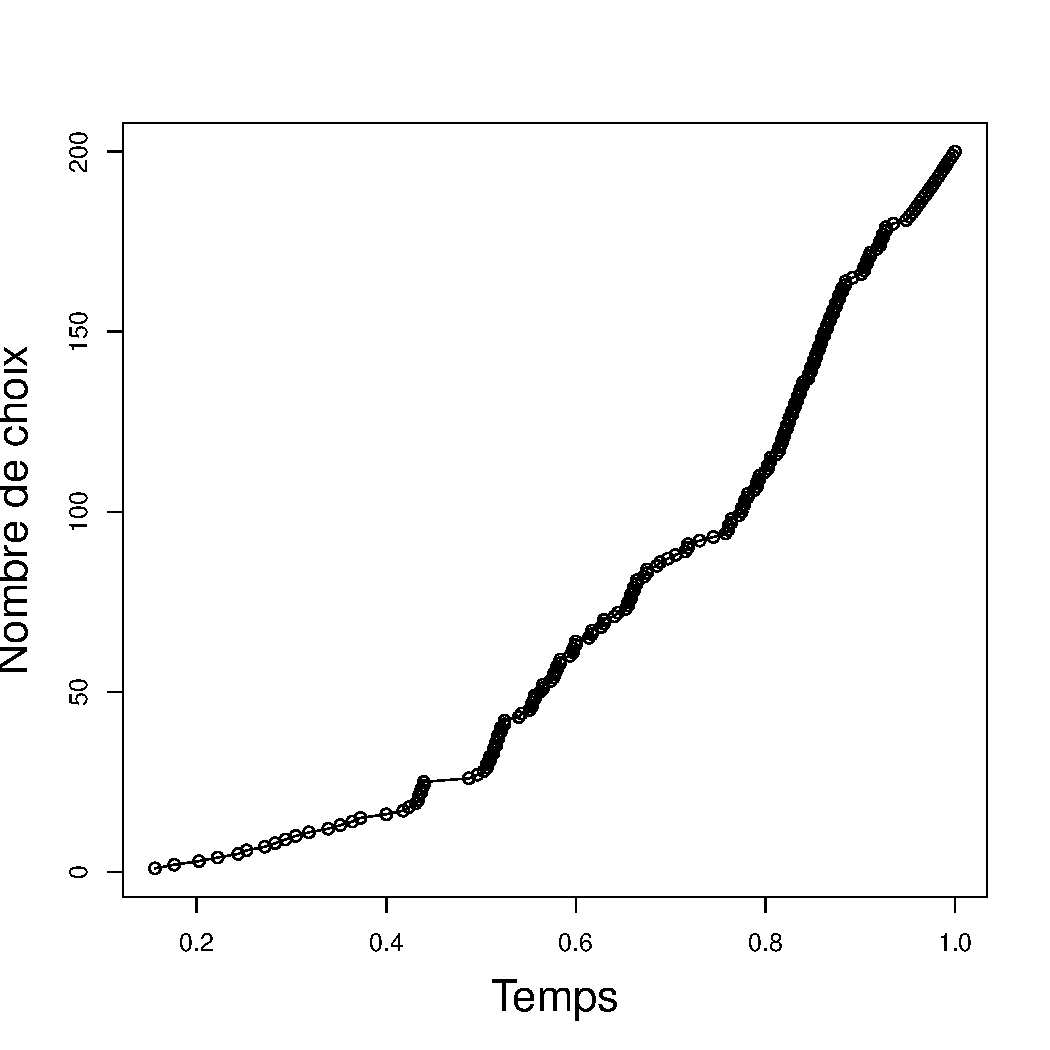
\includegraphics[width=0.27\textwidth,height=0.2\textheight]{figure/plot-soub-1} 
\end{knitrout}
    \vspace{-15pt}
    \caption{Affichage des données de l'expérience}
    \label{fig:donnees-soub}
\end{wrapfigure}

Ces données sont extraite du travail de thèse toujours en cours de Lola 
Soubeyrand. Il s'agit de l'enregistrement d'une expérience de type bandit 
consistant à choisir un bras selon les récompenses passées obtenues.

Nous allons seulement considérer les temps entre les choix pour réaliser notre 
analyse. Ces données sont présentées dans la figure~\ref{fig:donnees-soub}.

Aux vues de l'expérience, on peut s'attendre à une phase exploratoire des 
différents bras du bandit (phase d'\emph{exploration}) puis une fois le bras 
dont la stratégie convient au sujet trouvé à une concentration sur celui-ci (
phase d'\emph{exploitation}). Á noter qu'avec les évènements rares et extrême
des perturbations des convictions du sujet peuvent amener à des modifications du
comportement. Ces analyses \emph{a priori} nous invite à penser que l'on peut 
être dans le cas d'un processus de Poisson avec ruptures.



\begin{table}[!h]
    \centering
\begin{knitrout}
\definecolor{shadecolor}{rgb}{0.969, 0.969, 0.969}\color{fgcolor}
\begin{tabular}{rrrrrl}
\toprule
begin & end & Dt & DN & lambda & code.end\\
\midrule
0.00 & 0.16 & 0.16 & 0 & 6.21 & -\\
0.16 & 0.43 & 0.28 & 18 & 67.83 & -\\
0.43 & 0.44 & 0.01 & 7 & 595.14 & .\\
0.44 & 0.49 & 0.05 & 0 & 18.97 & -\\
0.49 & 0.68 & 0.19 & 59 & 310.93 & .\\
\addlinespace
0.68 & 0.76 & 0.08 & 9 & 113.51 & -\\
0.76 & 1.00 & 0.24 & 106 & 433.51 & .\\
\bottomrule
\end{tabular}

\end{knitrout}
    \caption{Résultats pour les données de \cite{soubeyrandDonneesTheseExperience2024}}
    \label{tab:resultat-soub-cv}
\end{table}

Et ainsi on trouve $\lambda = (0.1, 1.06, 9.28, 0.3, 4.85, 1.77, 6.76)$

En interpétant ces paramètres on peut voir deux premiers segments qui semblent
correspondre à la phase exploratoire initiale, puis une intensité de $9$ qui 
correspond à la première phase d'exploitation. Et par la suite une cassure dûe
à un évènement extrême négatif avant une reprise d'exploitation mixée à de 
l'exploration.

La détection de rupture pourra donc permettre d'analyser davantage les données 
d'autres sujets afin de voir si ce genre d'analyse peut fournir de plus amples
information sur la prise de décision en situation d'incertitude.

\newpage

\printbibliography
\nocite{*}

\end{document}
